\chapter{I$^2$C}
\label{chap:I2C}

This document shows all necessary transmissions which are needed for a successful interfacing on the I$^2$C bus. 

\section{ADC /MB}
\label{sec:ADC}

%\textbf{I$^2$C slave adress:\\
I$^2$C slave adress:\\
0b1001001 (0x49)

\subsection{Read}
\label{subsec:ADCread}

The read command get's the data from the adress, which is stored in the pointer register (blue colour). See figure \ref{fig:ADC1}

\begin{figure}[H]
	\centering\includegraphics[width=0.7\textwidth]{fig/ADC_read}
	\caption{Packages read ADC}
	\label{fig:ADC1}
\end{figure}


\subsection{Write}
\label{subsec:ADCwrite}



\begin{figure}[H]
	\centering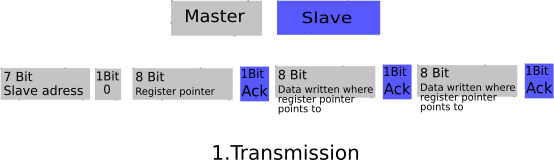
\includegraphics[width=0.7\textwidth]{fig/ADC_write}
	\caption{Packages write ADC}
	\label{fig:ADC2}
\end{figure}

\subsection{Read conversion register}
\label{subsec:ADCconversion}

To enable a read from a conversion register, several packages need to be sent. They can be seen in figure \ref{fig:ADC3}. All slave and master acknowledges are not shown because they are handled direct by the interface and so not important for the application.

\begin{figure}[H]
	\centering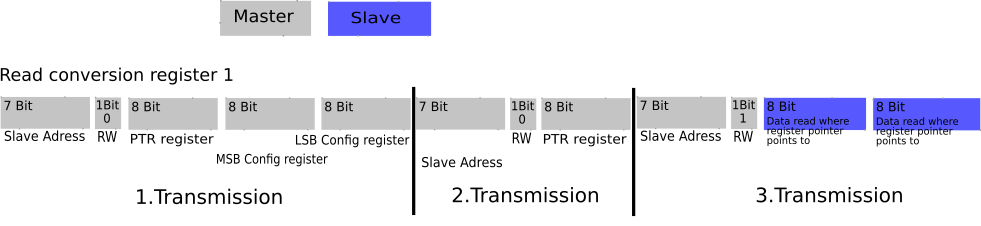
\includegraphics[width=1\textwidth]{fig/ADC_read_conversion}
	\caption{Packages conversion read ADC}
	\label{fig:ADC3}
\end{figure}

\section{Inertial Measurement Unit IMU}
\label{sec:ADC}

The Inertial measurement unit (IMU) has three different chips mounted. Each chip solves one of the measurements of this unit. Each chip has a different I$^2$C address. All slave and master acknowledges are not shown because they are handled direct by the interface and so not important for the application.

\subsection{Acceleration and Magnet Sensor}
\label{subsec:ACC}

\textbf{I$^2$C slave adress:\\
0b0011110}

There are several registers which have to be configured before reading and also several register where the acceleration, magnetic strength and if needed temperature can be read. To reduce the amount of pages of this document, they will be not listed here. All the registers can be found in the Datasheet 'IMU\_LSM303D.pdf', which is stored in the SVN directory '\textbackslash{}doc\textbackslash{}se\textbackslash{}Datasheets\textbackslash{}IMU'.

\subsubsection{Read}
\label{subsubsec:ACCread}

\begin{figure}[H]
	\centering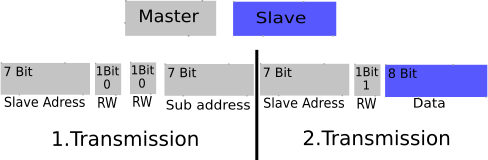
\includegraphics[width=0.7\textwidth]{fig/ACC_read_single}
	\caption{ACC read single data}
	\label{fig:ACC1}
\end{figure}

\begin{figure}[H]
	\centering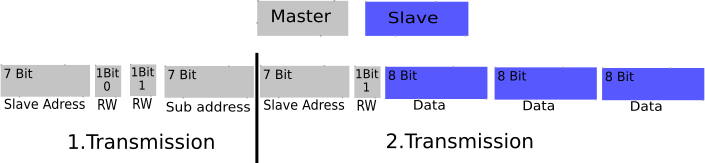
\includegraphics[width=1\textwidth]{fig/ACC_read_multiple}
	\caption{ACC read multiple data}
	\label{fig:ACC2}
\end{figure}

\textbf{1.Transmission: Slave address including RW bit ('0'): 0x3C}\\
\textbf{2.Transmission: Slave address including RW bit ('1'): 0x3D}


\subsubsection{Write}
\label{subsubsec:ACCwrite}

\begin{figure}[H]
	\centering\includegraphics[width=0.55\textwidth]{fig/ACC_write_single}
	\caption{ACC write single data}
	\label{fig:ACC3}
\end{figure}

\begin{figure}[H]
	\centering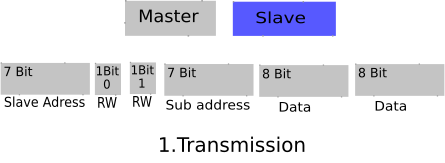
\includegraphics[width=0.7\textwidth]{fig/ACC_write_multiple}
	\caption{ACC write multiple data}
	\label{fig:ACC4}
\end{figure}

\textbf{1.Transmission: Slave address including RW bit ('0'): 0x3C}


\subsection{Gyroscope Sensor}
\label{subsec:Gyro}

\textbf{I$^2$C slave adress:\\
0b1101010}

There are several registers which have to be configured before reading and also several register where the rotational speed and if needed the temperature can be read. To reduce the amount of pages of this document, they will be not listed here. All the registers can be found in the Datasheet 'IMU\_L3GD20H.pdf', which is stored in the SVN directory '\textbackslash{}doc\textbackslash{}se\textbackslash{}Datasheets\textbackslash{}IMU'.

\subsubsection{Read}
\label{subsubsec:Gyroread}

\begin{figure}[H]
	\centering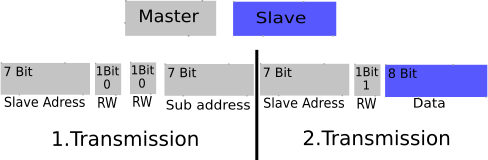
\includegraphics[width=0.7\textwidth]{fig/ACC_read_single}
	\caption{Gyro read single data}
	\label{fig:Gyro1}
\end{figure}

\begin{figure}[H]
	\centering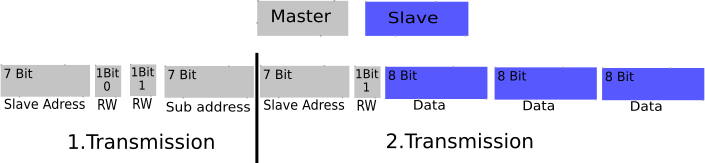
\includegraphics[width=1\textwidth]{fig/ACC_read_multiple}
	\caption{Gyro read multiple data}
	\label{fig:Gyro2}
\end{figure}

\textbf{1.Transmission: Slave address including RW bit ('0'): 0xD4}\\
\textbf{2.Transmission: Slave address including RW bit ('1'): 0xD5}

\subsubsection{Write}
\label{subsubsec:Gyrowrite}

\begin{figure}[H]
	\centering\includegraphics[width=0.55\textwidth]{fig/ACC_write_single}
	\caption{Gyro write single data}
	\label{fig:Gyro3}
\end{figure}

\begin{figure}[H]
	\centering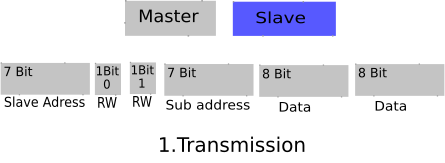
\includegraphics[width=0.7\textwidth]{fig/ACC_write_multiple}
	\caption{Gyro write multiple data}
	\label{fig:Gyro4}
\end{figure}

\textbf{1.Transmission: Slave address including RW bit ('0'): 0xD4}

\subsection{Pressure Sensor}
\label{subsec:Pressure}

\textbf{I$^2$C slave adress:\\
0b1011100}

There are several registers which have to be configured before reading and also several register where the pressure and if needed the temperature can be read. To reduce the amount of pages of this document, they will be not listed here. All the registers can be found in the Datasheet 'IMU\_LPS331AP.pdf', which is stored in the SVN directory '\textbackslash{}doc\textbackslash{}se\textbackslash{}Datasheets\textbackslash{}IMU'.

\subsubsection{Read}
\label{subsubsec:Pressureread}

\begin{figure}[H]
	\centering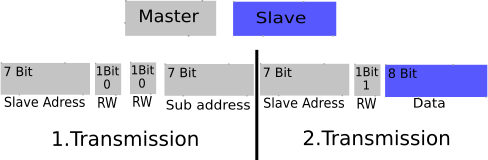
\includegraphics[width=0.7\textwidth]{fig/ACC_read_single}
	\caption{Pressure read single data}
	\label{fig:Pressure1}
\end{figure}

\begin{figure}[H]
	\centering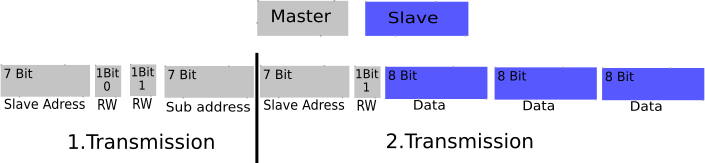
\includegraphics[width=1\textwidth]{fig/ACC_read_multiple}
	\caption{Pressure read multiple data}
	\label{fig:Pressure2}
\end{figure}

\textbf{1.Transmission: Slave address including RW bit ('0'): 0xB8}\\
\textbf{2.Transmission: Slave address including RW bit ('1'): 0xB9}

\subsubsection{Write}
\label{subsubsec:Pressurewrite}

\begin{figure}[H]
	\centering\includegraphics[width=0.55\textwidth]{fig/ACC_write_single}
	\caption{Pressure write single data}
	\label{fig:Pressure3}
\end{figure}

\begin{figure}[H]
	\centering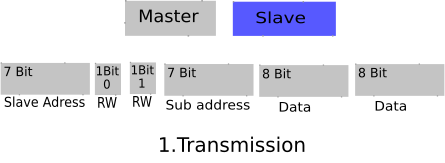
\includegraphics[width=0.7\textwidth]{fig/ACC_write_multiple}
	\caption{Pressure write multiple data}
	\label{fig:Pressure4}
\end{figure}

\textbf{1.Transmission: Slave address including RW bit ('0'): 0xB8}

\section{Motor Driver}
\label{sec:ADC}

All slave and master acknowledges are not shown because they are handled direct by the interface and so not important here. To enable flying with a Quadrocopter there are four motors and so four brushless drivers needed. Each of them has an individual address.

\pagebreak[3]{
\textbf{I$^2$C slave adress:\\
Motor 1  --> 0b0101001\\
Motor 2  --> 0b0101010\\
Motor 3  --> 0b0101011\\
Motor 4  --> 0b0101100}}

\subsection{Read}
\label{subsec:Motorread}

NOT DEFINED	

\subsection{Write}
\label{subsec:Motorwrite}

\begin{figure}[H]
	\centering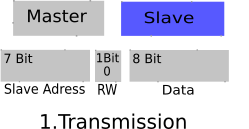
\includegraphics[width=0.4\textwidth]{fig/Motor_write}
	\caption{Motor write}
	\label{fig:Motor}
\end{figure}


\pagebreak[3]{
\textbf{1.Transmission: Slave address including RW bit ('0'):\\
Motor 1 --> 0x52\\
Motor 2 --> 0x54\\
Motor 3 --> 0x56\\
Motor 4 --> 0x58}}

\textbf{Possible Data values are in the range of 10 (Decimal) up to 255 (Decimal). So in the range from 0x0A to 0xFF.}